\documentclass[11pt,a4paper]{article}
\usepackage[utf8]{inputenc}
\usepackage[a4paper]{geometry}

\usepackage[english]{babel}
\hyphenation{sil-la-ba-zio-ne pa-ren-te-si}
\usepackage{newlfont}

\usepackage{amsmath}
\usepackage{amsfonts}
\usepackage{amssymb}
\usepackage{amsthm}
\usepackage {amsmath, amssymb}
\usepackage{bbm}

\usepackage{graphicx}
\usepackage{rotating}
\usepackage{subfigure}
\usepackage{lscape}
\usepackage[bf, scriptsize]{caption}
\usepackage{multirow}
\usepackage{longtable}
\hyphenation{Low-din}
\usepackage{titling}
\usepackage{eurosym}
\usepackage{adjustbox}

% included by Nicola for correct highlighting of C++ code
\usepackage{listings}
\usepackage{xcolor}

\definecolor{dkgreen}{rgb}{0,0.6,0}
\definecolor{dred}{rgb}{0.545,0,0}
\definecolor{dblue}{rgb}{0,0,0.545}
\definecolor{lgrey}{rgb}{0.9,0.9,0.9}
\definecolor{gray}{rgb}{0.4,0.4,0.4}
\definecolor{darkblue}{rgb}{0.0,0.0,0.6}

\lstdefinelanguage{cpp} {
  backgroundcolor=\color{lgrey},
  basicstyle=\footnotesize \ttfamily \color{black} \bfseries,
  breakatwhitespace=false,
  breaklines=true,
  captionpos=b,
  commentstyle=\color{dkgreen},
  deletekeywords={...},
  escapeinside={\%*} {*)},
  frame=single,
  language=C++,
  keywordstyle=\color{purple},
  morekeywords={BRIEFDescriptorConfig,string,TiXmlNode,DetectorDescriptorConfigContainer,istringstream,cerr,exit},
  identifierstyle=\color{black},
  stringstyle=\color{blue},
  numbers=left,
  numbersep=5pt,
  numberstyle=\tiny\color{black},
  rulecolor=\color{black},
  showspaces=false,
  showstringspaces=false,
  showtabs=false,
  stepnumber=1,
  tabsize=2,
  title=\lstname,
}
% end inclusion

\author{F. Cinus \& F. Delussu \& N. Sella}
\title{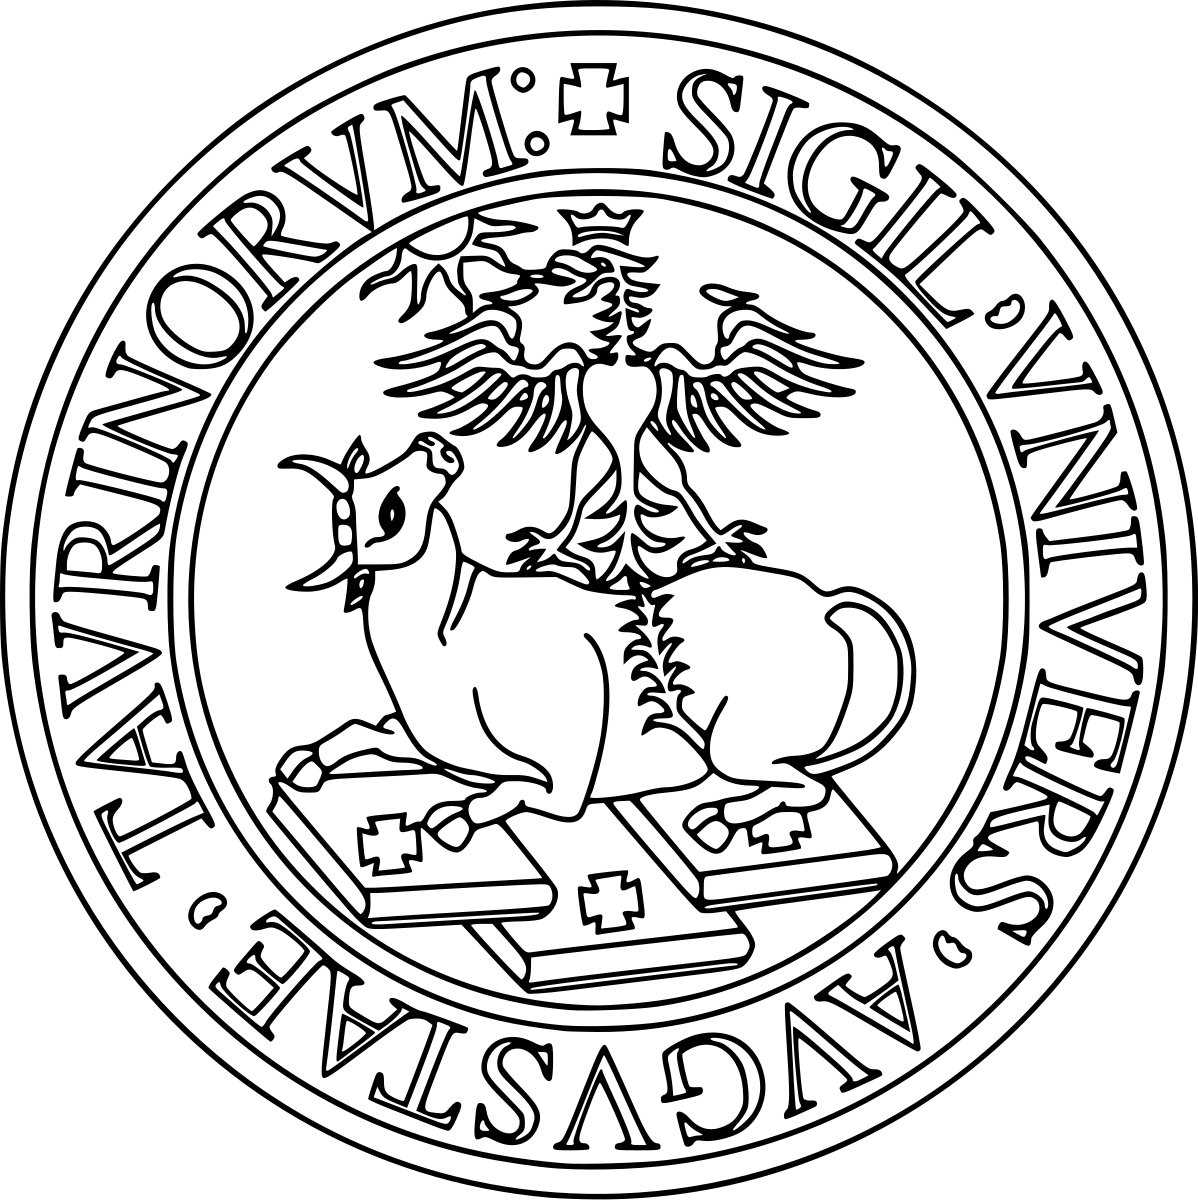
\includegraphics[scale=0.12]{Unito-logo} \\ \LARGE{UNIVERSIT\`{A} DEGLI STUDI DI TORINO}
  \\
  TANS Course A.A. 2017/2018 Prof. Massimo Masera
  \\
  \textbf{Ising Model Simulation with Monte Carlo methods}
}

\begin{document}



\section*{Classes}
	
\subsection*{Lattice}

The Lattice class permits to construct a Lattice, compute its termodynamic quantities 
and change its state with the Metropolis Algorithm. \\	  
Computation details of functions such as \textbf{energy}() and \textbf{cooling}() are thoroughly explained in Model section. \\ 

\begin{itemize}

	\item[] 
	PRIVATE DATA MEMBERS \\ 
	
	\begin{tabular}{lll}
		const uint 		& \textbf{N}        & number of spins along one edge				  \\
		const uint 		& \textbf{dim}      & dimension										   \\
  		const uint 		& \textbf{num\textunderscore spin} & total number of spins : $N^{dim}$  \\
  		bool ${}^*$  	& \textbf{lattice}  & boolean array of size \textbf{num\textunderscore spin} \\
  		static double 	& \textbf{T}        & temperature  										  	  \\
	\end{tabular}
	\\

	\item[] 
	PUBLIC MEMBER FUNCTIONS \\ 
	\begin{itemize}
		\item[] CONSTRUCTORS \\

			\item[] \textbf{Lattice}()	 
			\begin{itemize}
				\item[] Default Constructor \\ 
						Creates Lattice object with N=1 , dim=1 \\
						The single entry of \textbf{lattice} is set to 0 or 1 with 0.5 probability   
			\end{itemize}
			
			\item[] \textbf{Lattice}(const uint\& \textunderscore N , const uint\& \textunderscore dim)	 
			\begin{itemize}
				\item[] Standard Constructor \\
						Creates Lattice object with N = \textunderscore N,  dim = \textunderscore dim \\
						Sets each \textbf{lattice} entry to 0 or 1 with 0.5 probability 
			\end{itemize}
			
			\item[] \textbf{Lattice}(const Lattice\& obj)		 
			\begin{itemize}
				\item[] Copy Constructor \\
						Creates Lattice object with obj's data members \\
			\end{itemize}

		
		\item[]
		DESTRUCTOR \\
		
			\item[] \textbf{$\sim$ Lattice}	 
			\begin{itemize}
				\item[] Frees up memory allocated by \textbf{lattice} \\
			\end{itemize}		
		
\newpage 		
	
		\item[] 
		PHYSICAL AND NUMERICAL FUNCTIONS \\
 		
			\item[] bool \textbf{flipSpin}(const uint\& n)		 
			\begin{itemize}
				\item[] If n $<$ \textbf{num\textunderscore spin} \\
				Sets \textbf{lattice}[n] to !\textbf{lattice}[n] and returns true \\
				Else it doesn't change \textbf{lattice} and returns false 
						
			\end{itemize}

			\item[] int \textbf{dE}(const uint\& n) const		 
			\begin{itemize}
				\item[] Returns energy variation resulting from applying \textbf{flipSpin}(n) \\
						{\small
						\textsf{n.b.} : it's a const method, it doesn't apply \textbf{flipSpin}(n)
						} 
			\end{itemize}
			
			\item[] int \textbf{energy}() const;		 
			\begin{itemize}
				\item[] Returns total Energy 
			\end{itemize} 
			
			\item[] float \textbf{magnetization}() const		 
			\begin{itemize}
				\item[] Returns Magnetization per site  
				
			\end{itemize}
			
			\item[] void \textbf{cooling}(const uint\& iter) 		 
			\begin{itemize}
				\item[] Applies one step of Metropolis Algorithm 
			\end{itemize}
			
			
			\item[] void \textbf{cooling}(const uint\& iter) 		 
			\begin{itemize}
				\item[] Applies \textbf{iter} steps of Metropolis Algorithm
			\end{itemize}
			
			\item[] double * \textbf{coolingPar}()	 
			\begin{itemize}
				\item[] Applies \textbf{cooling}() and returns a four-dimensional array \textbf{arr} \\
						\textbf{arr} are respectively variations of : \\
						Temperature , Energy , Magnetization , Energy per site  \\
			\end{itemize}
		
		\item[] 
		OVERLOADED OPERATORS \\

			\item[] Lattice\& \textbf{operator=}(const Lattice\& obj)		 
			\begin{itemize}
				\item[] Assignment operator \\
			\end{itemize}
			
			\item[] friend std::ostream\& \textbf{operator$<<$}(std::ostream\& out, const Lattice\& lat) 	
			\begin{itemize}
				\item[] Taking \textsf{lat} as a reference to a Lattice object \\
				Prints \textbf{lattice} member of \textsf{lat} by typing the command \textsf{cout $<<$ lat ;} 
			\end{itemize}	
			
			\item[] bool \textbf{operator==}(const Lattice\& obj) 		 
			\begin{itemize}
				\item[] Taking \textsf{lat1} and \textsf{lat2} as references to Lattice objects \\
						\textsf{lat1 == lat2} returns true if \textsf{lat1} and \textsf{lat2} have same data members
			\end{itemize}
			
\newpage			
			
		\item[] 
		GETTERS AND SETTERS \\
					
			\item[] uint \textbf{getN}() const ; uint \textbf{getDim}() const; uint \textbf{getNumSpin}() const 	
			\begin{itemize}
			\item[] returns respectively \textbf{N} , \textbf{dim} , \textbf{num\textunderscore spin} 
			\end{itemize}			
			
			\item[] bool \textbf{getSpin}(const uint \& n) const 		 
			\begin{itemize}
				\item[] returns \textbf{lattice}[n] entry
			\end{itemize}
					
			\item[] double \textbf{getT}() ; static void \textbf{setT}(const double\& \textunderscore T)	
			\begin{itemize}
				\item[] respectively : \\ 
						Returns \textbf{T} ; Sets \textbf{T} = \textunderscore T \\
			\end{itemize}
			
		\item[] 
		OTHERS \\
			
			\item[] void \textbf{printLatticeCSV}(const TString\& name) const		 
			\begin{itemize}
				\item[] prints \textbf{lattice} in a csv file saved in the working directory
			\end{itemize}
			
			\item[] 
			{\small			
			void \textbf{printLatticeROOT}(const TString\& name , const TString\& ln = "lat") const	
			}			
			\begin{itemize}
				\item[] saves Lattice object in a root file 
			\end{itemize}
			
	\end{itemize}

	
\end{itemize}

\newpage

\subsection*{DrawLattice}

DrawLattice class permits to draw a 2D or 3D Lattice inside a TCanvas \\
The Lattice object to be drawn can be imported in two ways with two Constructors \\
The first constructor takes a Lattice object as argument \\
The second constructor takes the name of a root file and the name of a Lattice saved with the \textbf{printLatticeROOT} method \\
The Lattice is displayed in a TMultiGraph which has two TGraphs for up and down spins, with respectively kRed and kBlue color. \\ 
The computation of the spin coordinates is explained in the Model Section. 
         
\begin{itemize}

	\item[] PRIVATE DATA MEMBERS \\ 
	
	\begin{tabular}{lll}
		Lattice & \textbf{lattice}  & Lattice object \\
		
  		uint  & \textbf{N}, \textbf{ dim}, \textbf{ num\textunderscore spin} 
  		& \textbf{N}, \textbf{ dim}, \textbf{ num\textunderscore spin} of \textbf{lattice} \\
  		
		TString & \textbf{fname} & name of root file \\
		TString & \textbf{lname} & name of \textbf{Lattice} saved in root file fname\\
		TString & \textbf{cname} , \textbf{ctitle} & Tcanvas name and title \\
		TString & \textbf{gname} , \textbf{gtitle} & TMultiGraph name and title \\		   			
	\end{tabular}
	
	\begin{itemize}
	\item[]	{\small
		\textbf{cname}, \textbf{ctitle}, \textbf{gname}, \textbf{gtitle} 
		are assigned the same way in each of the three Constructors as 
		\textsf{ : cname("cv"), ctitle("default canvas"), gname("gr"), gtitle("Ising")} 
		} 
		\\
	\end{itemize}
		
	\item[] PUBLIC MEMBER FUNCTIONS \\ 
	\begin{itemize}
		\item[] CONSTRUCTORS \\

			\item[] \textbf{DrawLattice}()		 
			\begin{itemize}
				\item[] Default Constructor \\
						Creates lattice with Lattice Standard Constructor					
						
			\end{itemize}
			
			\item[] \textbf{DrawLattice}(const Lattice\& lat)		 
			\begin{itemize} 
				\item[] First Standard Constructor \\
						Sets \textbf{lattice} = lat 
						   
			\end{itemize}
			
			\item[] \textbf{DrawLattice}(const TString\& \textunderscore fname, const TString\& 														\textunderscore lname)		 
			\begin{itemize}
				\item[] Second Standard Constructor \\
						Searches a Tfile with name \textunderscore fname \\
						Sets \textbf{lattice} with \textbf{readFile}() 						
				{\small
						\item[] void \textbf{readFile}()
						\begin{itemize}
							\item[] Gets Lattice object with name \textunderscore lname 
									from the TFile and sets it to \textbf{lattice}				   		
						\end{itemize}						 
				}		 
			\end{itemize}
			
\newpage
						
		\item[] DRAW FUNCTION \\
		
			\item[] void \textbf{draw}()		 
			\begin{itemize}
				\item[] performs a switch statement on \textbf{dim} \\  
						if \textbf{dim} = 2 applies \textbf{draw2D}() \\
						if \textbf{dim} = 3 applies \textbf{draw3D}() \\						    
						else returns without applying a draw Function  
			\end{itemize}

		\item[]	GETTERS \\
				
			\item[] uint \textbf{getN}() ; uint \textbf{getDim}() ; uint \textbf{getNumSpin}()  	
			\begin{itemize}
			\item[] returns respectively \textbf{N}, \textbf{dim}, \textbf{num\textunderscore spin} 
			\end{itemize}	
			
	\end{itemize}
	
	\item[] PRIVATE MEMBER FUNCTIONS \\ 
	\begin{itemize}
			
		\item[] DRAW FUNCTIONS
			\item[] void \textbf{draw2D}()		 
			\begin{itemize}
				\item[] draws a bidimensional TMultiGraph
			\end{itemize}
			
			\item[] void \textbf{draw3D}()  		 
			\begin{itemize}
				\item[] draw a threedimensional TMultiGraph
			\end{itemize}
			
		\item[] SETTERS
			
			\item[] void \textbf{setN}() ; void \textbf{setDim}() ; void \textbf{setNumSpin}()				
			\begin{itemize}
				\item[]
						{\small
						 Sets \textbf{N}, \textbf{dim}, \textbf{num\textunderscore spin} respectively to 
						\textbf{lattice.N}, \textbf{lattice.dim}, \textbf{lattice.num\textunderscore spin} 
						\\
						\textsf{n.b.}
						applied in First and Second Standard Constructor after \textbf{lattice} is set 
						}
			\end{itemize}
			
			\item[] void \textbf{setN}(\textunderscore N) ;
					void \textbf{setDim}(\textunderscore dim) ;
					void \textbf{setNumSpin}(\textunderscore num\textunderscore spin ) 	
			\begin{itemize}
				\item[] Sets \textbf{N}, \textbf{dim}, \textbf{num\textunderscore spin} respectively to 
						\textunderscore N, \textunderscore dim, \textunderscore num\textunderscore spin
			\end{itemize}	
				
	\end{itemize}

	
\end{itemize}

\newpage


\subsection*{SimulationLattice}

Simulation Lattice permits to run a simulation and collect data during runtime.
The simulation is performed on a set of Lattice objects over a range of temperatures \\
All Lattices have same edge length and same dimension
For each temperature :  
\begin{itemize}
	\item[] each Lattice is submitted to \textbf{I0} cooling iterations in order to reach thermal equilibrium. \\ In this step data are not collected
	\item[] each Lattice is submitted to \textbf{iter} cooling iterations,   \\
	 		during each iteration measures of temperature, energy, magnetization and susceptibility are 				collected. 
\end{itemize} 
 
\begin{itemize}

	\item[] PRIVATE DATA MEMBERS \\ 
	
	\begin{tabular}{lll}
		Lattice ${}^*$  	& \textbf{lattice\textunderscore vector}  & vector storing a Lattice for each entry\\
			
		const uint 		& \textbf{N}        & edge length of each Lattice \\
		const uint 		& \textbf{dim}      & dimension of each Lattice		\\
		const uint 		& \textbf{dim\textunderscore vector}    & dimension of \textbf{lattice\textunderscore vector} \\
		
  		const TString  	& \textbf{file} & root file name in which data are collected \\
  		
  		uint & \textbf{I0} & number of iterations not collecting data \\
		uint 		& \textbf{iter} & number of iterations collecting data \\
  										
  		double 	& \textbf{tempmin}        & minimum range's temperature  \\
  		double 	& \textbf{tempmax}        & maximum range's temperature	  \\
  		uint 	& \textbf{tempstep}       & number of temperatures in the range \\
   		
	\end{tabular}
	\item[] \textbf{n.b.} : \textbf{tempstep} should be a multiple of 4 for implementation reasons \\ 

	\item[] PUBLIC MEMBER FUNCTIONS \\ 
	\begin{itemize}
		\item[] CONSTRUCTORS \\

			\item[] \textbf{SimulationLattice}()	 
			\begin{itemize}
				\item[] Default Constructor
			\end{itemize}
			
			\item[] \textbf{SimulationLattice}(const uint\& \textunderscore N, const uint\& \textunderscore dim, const uint\& \textunderscore dim\textunderscore vector)		 
			\begin{itemize}
				\item[] 3-Parameters Constructor \\
						The other data members can be assigned with the setter methods
			\end{itemize}
			
			\item[] \textbf{SimulationLattice}(const uint\& \textunderscore N, const uint\& \textunderscore dim, const uint\& \textunderscore dim\textunderscore vector, const TString\& \textunderscore file, const uint\& \textunderscore i0, const uint\& \textunderscore iter, const double\& \textunderscore tempmin, const double\& \textunderscore tempmax, const uint\& \textunderscore tempstep)		 
			\begin{itemize}
				\item[] Full Parameter Constructor
			\end{itemize}

			\item[] \textbf{SimulationLattice}(const Lattice\& \textunderscore lat , const uint\& \textunderscore dim\textunderscore vector, const TString\& \textunderscore file, const uint\& \textunderscore i0, const uint\& \textunderscore iter, const double\& \textunderscore tempmin, const double\& \textunderscore tempmax, const uint\& \textunderscore tempstep)			 
			\begin{itemize}
				\item[] Constructor based on a Lattice  \\
						Sets \textbf{N} and \textbf{dim} as those of lat    
			\end{itemize}
			
			\item[] \textbf{SimulationLattice}(const SimulationLattice\& obj)		 
			\begin{itemize}
				\item[] Copy Constructor
			\end{itemize}
			
			\item[] SimulationLattice\& \textbf{operator=}(const SimulationLattice\& obj)		 
			\begin{itemize}
				\item[] Assignment Operator \\
			\end{itemize}
		
		\item[] DESTRUCTOR \\
		
			\item[] \textbf{$\sim$ SimulationLattice}	 
			\begin{itemize}
				\item[] Frees up memory allocated by \textbf{lattice\textunderscore vector}  \\
			\end{itemize}
			
		\item[] RUN FUNCTION \\
			
			\item[] void \textbf{run}() const		 
			\begin{itemize}
				\item[] Performs the simulation \\  
			\end{itemize}
						
		
		\item[] GETTERS AND SETTERS \\
 			
 			\item[] Getters methods are defined for all the Private Data Members except for \textbf{lattice\textunderscore vector}, but its entries can be obtained with : 
 			  
 			\item[] Lattice \textbf{getLattice}(const uint\& i)		 
			\begin{itemize}
				\item[] returns \textbf{lattice\textunderscore vector}[i]  
			\end{itemize}
 					
 			\item[] Setters methods are defined for all the Private Data Members except for \textbf{lattice\textunderscore vector} \textbf{N}, \textbf{dim} and \textbf{dim\textunderscore vector}   
 			 		
	\end{itemize}

	
\end{itemize}

\newpage

\subsection*{AnalysisLattice}

AnalysisLattice performs an analysis on raw data collected on a simulation input-file \\ 
The analysis creates an output-file which stores : 
\begin{itemize}
	\item[] mean and standard deviation of physical quantities for each Lattice and temperature of the
	 		simulation.
	\item[] mean and standard deviation performed over the Lattices for each temperature of the simulation 	 		
	 		 
\end{itemize}
Once the output file is created, the physical functions can be plotted into a graph \\
The curves of Magnetization and Susceptibility vs Temperature can be fitted in order to estimate the Critical Temperature and Exponenents of the phase transition.


\begin{itemize}

\item[] PRIVATE DATA MEMBERS \\

  \begin{tabular}{lll}
    const TString               & \textbf{file\textunderscore in}      & input root file name    \\
    const TString               & \textbf{file\textunderscore out}      & output root file name  \\
    % bisogna decidere se togliere o meno questo data member se fittiamo il lattice
    static double       & \textbf{TempCritic}   & critic temperature                                            \\
  \end{tabular}

\item[] PUBLIC MEMBER FUNCTIONS \\
  \begin{itemize}
  \item[] CONSTRUCTOR \\

  \item[] \textbf{AnalysisLattice}(const TString\& file\textunderscore input, const TString\& file\textunderscore output)
    \begin{itemize}
    \item[] Parametric Constructor\\
      Sets input and output file names.
    \end{itemize}

  \item[] RUN FUNCTION

  \item[] void \textbf{run}()
    \begin{itemize}
    \item[] Performs the analysis of the previous simulation.\\
      Recreates output file.
    \end{itemize}

  \item[] DRAW FUNCTIONS

  \item[] TGraphErrors ${}^*$ \textbf{drawLattice}(cuint\& lattice\textunderscore number,
    cuint\& x\textunderscore axis,
    cuint\& y\textunderscore axis)
    \begin{itemize}
    \item[]
    \end{itemize}

  \item[] TGraphErrors ${}^*$ \textbf{drawLatticeMean}(
    cuint\& x\textunderscore axis,
    cuint\& y\textunderscore axis)
    \begin{itemize}
    \item[]
    \end{itemize}

  \item[] TGraphErrors ${}^*$ \textbf{draw}(
    cuint\& x\textunderscore axis,
    cuint\& y\textunderscore axis)
    \begin{itemize}
    \item[] 
    \end{itemize}

\newpage

  \item[] FIT FUNCTIONS \\

  \item[] static double \textbf{analiticX}(double $*$ x, double $*$ par)
    \begin{itemize}
    \item[]
    \end{itemize}

  \item[] static double \textbf{analiticM}(double $*$ x, double $*$ par)
    \begin{itemize}
    \item[]
    \end{itemize}

  \item[] void \textbf{findTcritic}()
    \begin{itemize}
    \item[]
    \end{itemize}

  \item[] void \textbf{fitLattice}( bool mean,
    cuint\& x\textunderscore axis,
    cuint\& y\textunderscore axis,
    double Tc,
    double fit\textunderscore temp\textunderscore min,
    double fit\textunderscore temp\textunderscore max,
    int lat\textunderscore number
    );
    \begin{itemize}
    \item[]
    \end{itemize}


  \item[]       GETTERS AND SETTERS \\

  \item[] static double \textbf{getTempCritic}()
    \begin{itemize}
    \item[] Get critic temperature.
    \end{itemize}

  \item[] static void \textbf{setTempCritic}(const double\& \textunderscore TempCritic);
    \begin{itemize}
    \item[] Set critic temperature.
    \end{itemize}

  \item[] TString \textbf{getFileIn}() const;
    \begin{itemize}
    \item[] Get input file name.
    \end{itemize}

  \item[] TString \textbf{getFileOut}() const
    \begin{itemize}
    \item[] Get output file name.
    \end{itemize}

  \item[]  void \textbf{setFileIn}(const TString\& file\textunderscore input)
    \begin{itemize}
    \item[] Set input file name.
    \end{itemize}

  \item[] void \textbf{setFileOut}(const TString\& file\textunderscore out)
    \begin{itemize}
    \item[] Set output file name.
    \end{itemize}

  \end{itemize}
\end{itemize}

\newpage

\lstinputlisting[language=cpp, caption={Caption}]
{../test/relationMacro.C}




\end{document}
